\section{Massless Symmetric Tensor Exchange\label{SecMasslessTen4}}
%%%%%%%%%%%%%%%%%%%%%%%%%%%%%%%%%%%%%%%%%%%%%%%%%%%%%%%%%%%%%%%%%%%%%%%%%%%%%%%%%%%%%%%%%
The next natural step is the case when the external matter particles exchange massless symmetric tensor quanta. We consider a system that is equivalent to particles interacting via linearized gravity.

The interaction term for scalar particles coupled to a symmetric tensor field $h_{mn}$ is
\begin{equation}
	S_{\text{int}}[q_{a}, q_{b}, h] \equiv \frac{1}{2} \int \mathrm{d}\tau \, \dot{q}_{a}^{m} \dot{q}_{a}^{n} h_{mn}[q_{a}(\tau)] + \frac{1}{2} \int \mathrm{d}\sigma \, \dot{q}_{b}^{m} \dot{q}_{b}^{n} h_{mn}[q_{b}(\sigma)] \label{SintTen}
\end{equation}
We follow the same steps as in previous sections. Start with the two-body path integral
\begin{equation}
	\mathcal{G}_{h}[h] \equiv \int\limits_{x_{1}}^{x_{3}} \mathrm{D}q_{a}(\tau) \int\limits_{x_{2}}^{x_{4}} \mathrm{D}q_{b}(\sigma) \, \exp{\left(- i S_{0}[q_{a}, q_{b}] - i S_{\text{int}}[q_{a}, q_{b}, h] \right)}
\end{equation}
and integrate over the field $h$ to obtain the ``effective'' two-body path integral
\begin{equation}
	\mathcal{F}_{h}(3,4|1,2) \equiv \int \mathrm{D}h_{mn}(x) \, \mathcal{G}_{h}[h] \exp{\left( -i S_{\text{kin}}[h] \right)}
\end{equation}
where $S_{\text{kin}}$ is the (linearized) gauge-fixed kinetic term
\begin{equation}
	S_{\text{kin}}[h] = \frac{1}{2g_{2}^{2}} \int \int \mathrm{d} x \mathrm{d}y \left[ h_{mp}(x) (K_{2})^{mnpq} h_{nq}(y) \right] \label{SkinTen}
\end{equation}
with
\begin{equation}
\begin{split}
	(K_{2})^{mnpq}(x|y) \equiv {}& \delta(x - y) \\
	&\times \left[ \frac{1}{2} \eta^{mn} \eta^{pq} + \frac{1}{2} \eta^{mq} \eta^{np} - \frac{1}{2} \left(2 - \frac{1}{\xi_{2}} \right) \eta^{mp} \eta^{nq} \right] \\
	&\times \left(- \frac{1}{2} \partial^{2} \right) \\
	&+ \delta(x - y) \left(1 - \frac{1}{\xi_{2}} \right) \\
	&\times \left( \frac{1}{2} \eta^{mn} \partial^{p} \partial^{q} + \frac{1}{2} \eta^{mq} \partial^{n} \partial^{q} - \eta^{mp} \partial^{n} \partial^{q} \right)
\end{split}
\end{equation}
In the Fermi-Feynman gauge ($\xi_{2} = 1$) we have
\begin{equation}
	(K_{2})^{mnpq}(x|y) = \frac{1}{2} \left(\eta^{mn} \eta^{pq} + \eta^{mq} \eta^{np} - \eta^{mp} \eta^{nq} \right) K_{0}(x|y)
\end{equation}
After integrating over $h$ and ignoring the self-interactions, we find
\begin{equation}
	\mathcal{F}_{h}(3,4|1,2) = \int\limits_{x_{1}}^{x_{3}} \mathrm{D}q_{a}(\tau) \int\limits_{x_{2}}^{x_{4}} \mathrm{D}q_{b}(\sigma) \, \exp{\left(- i S_{0}[q_{a}, q_{b}] + i S_{2}^{h}[q_{a}, q_{b}] \right)}
\end{equation}
where the free term is given by (\ref{FreeS}) and the two-body interaction term is
\begin{equation}
	S_{2}^{h} = \frac{g_{2}^{2}}{8} \int \int  \mathrm{d}\tau \mathrm{d}\sigma \left[ 2 \left[ \dot{q}_{a}(\tau) \cdot \dot{q}_{b}(\sigma) \right]^{2} - \dot{q}_{a}^{2}(\tau) \dot{q}_{b}^{2}(\sigma) \right] G_{0}\left[q_{a}(\tau) | q_{b}(\sigma) \right] \label{Sh}
\end{equation}

In section \ref{SecDimAn} we found that the coupling parameter $g_{2}$ has units
\begin{equation}
	\left[g_{2} \right] = \left( \frac{2 - D}{2} \right) \left[ \text{mass} \right]
\end{equation}
When $D = 4$, we have that $g_{2}$ has units of inverse mass (the Planck length). So we write
\begin{equation}
	g_{2}^{2} = \frac{8\alpha_{2}}{2 \pi} \mu^{(4 - D)}
\end{equation}
where $\mu$ has units of mass and $\sqrt{\alpha_{2}}$ has units of inverse mass. Similarly, in $D = 3$ we have that $g_{2}^{2}$ has units of inverse mass. We write
\begin{equation}
	g_{2}^{2} = \frac{8 \beta_{2}}{(2 \pi)^{3/2}} \mu^{(3 - D)}
\end{equation}
where $\mu$ has units of mass and $\beta_{2}$ has units of inverse mass.
%%%%%%%%%%%%%%%%%%%%%%%%%%%%%%%%%%%%%%%%%%%%%%%%%%%%%%%%%%%%%%%%%%%%%%%%%%%%%%%%%%%%%%%%%
\subsection{Eikonal Van Vleck Function}
%%%%%%%%%%%%%%%%%%%%%%%%%%%%%%%%%%%%%%%%%%%%%%%%%%%%%%%%%%%%%%%%%%%%%%%%%%%%%%%%%%%%%%%%%
Since the pre-factor in (\ref{Sh}) only depends on the slopes of the path functions, in the eikonal JWKB approximation we have a familiar situation. At the eikonal paths (\ref{eikConf2}) we find
\begin{align}
	\Sigma_{2}^{h} &\equiv S_{2}^{h}\left[e_{a}, e_{b} \right] \nonumber \\
	&= \frac{g_{2}^{2}}{8} \int \int \mathrm{d}\tau \mathrm{d}\sigma \left[ 2 \left[ \dot{e}_{a}(\tau) \cdot \dot{e}_{b}(\sigma) \right]^{2} - \dot{e}_{a}^{2}(\tau) \dot{e}_{b}^{2}(\sigma) \right] G_{0}\left[e_{a}(\tau) | e_{b}(\sigma) \right] \nonumber \\
	&= -\frac{i \alpha_{2}}{2 \pi} \left[ \frac{2(x_{31} \cdot x_{42})^{2} - x_{31}^{2} x_{42}^{2}}{T_{a}^{2} T_{b}^{2}} \right] \Upsilon
\end{align}
with $\Upsilon$ given by (\ref{upsi}). In the eikonal JWKB approximation we use (\ref{upsi2}) and obtain
\begin{equation}
\begin{split}
	\Sigma_{2}^{h} \approx {}&{- i \alpha_{2}} \left[ \frac{2(x_{31} \cdot x_{42})^{2} - x_{31}^{2} x_{42}^{2}}{T_{a} T_{b} \sqrt{x_{31}^{2} x_{42}^{2} - (x_{31} \cdot x_{42})^{2}} } \right] \\
	&\times \Gamma\left( \frac{D - 4}{2} \right) \left( \frac{2}{\mu^{2} B_{12}^{2}} \right)^{(D - 4)/2}
\end{split}
\end{equation}
Using $D = 4 + 2 \epsilon$ and introducing
\begin{equation}
	\rho_{2} \equiv \frac{2(x_{31} \cdot x_{42})^{2} - x_{31}^{2} x_{42}^{2}}{T_{a} T_{b} \sqrt{x_{31}^{2} x_{42}^{2} - (x_{31} \cdot x_{42})^{2}} } \label{rho2Def}
\end{equation}
we can write more compactly
\begin{equation}
	\Sigma_{2}^{h} \approx -i \alpha_{2} \rho_{2} \Gamma(\epsilon) \left( \frac{2}{\mu^{2} B_{12}^{2}} \right)^{\epsilon}
\end{equation}
which has a by-now-familiar form. Note that, unlike $\rho_{1}$ (but similar to $\rho_{0}$), the quantity $\rho_{2}$ depends on the worldline moduli.
%%%%%%%%%%%%%%%%%%%%%%%%%%%%%%%%%%%%%%%%%%%%%%%%%%%%%%%%%%%%%%%%%%%%%%%%%%%%%%%%%%%%%%%%%
\subsection{Eikonal S-Matrix}
%%%%%%%%%%%%%%%%%%%%%%%%%%%%%%%%%%%%%%%%%%%%%%%%%%%%%%%%%%%%%%%%%%%%%%%%%%%%%%%%%%%%%%%%%
We follow the same steps as in \S\ref{SMatrixMasslessSca} and \S\ref{SMatrixVec}. After integrating over $X$, $x_{31}$ and $x_{42}$, the function $\rho_{2}$ becomes
\begin{equation}
	\rho_{2} = \frac{2(p_{31} \cdot p_{42})^{2} - p_{31}^{2} p_{42}^{2}}{\sqrt{p_{31}^{2} p_{42}^{2} - (p_{31} \cdot p_{42})^{2}}}
\end{equation}
Similar considerations as before lead to the following truncated on-shell scattering amplitude
\begin{equation}
\begin{split}
	\widehat{\mathcal{A}}_{h} = {}& \mathcal{A}_{\text{tree}}^{h}(s, t, u) \\
	&\times \sum_{L = 0}^{\infty} \frac{\left[\alpha_{2} \rho_{2}(s, u) \right]^{L}}{\Gamma(L + 1)} \frac{\Gamma(1 + \epsilon) [\Gamma(\epsilon)]^{L} \Gamma(1 - L \epsilon)}{\Gamma(1 + \epsilon + L \epsilon)} \left( -\frac{t}{2 \mu^{2}} \right)^{L \epsilon}
\end{split} \label{hatATen}
\end{equation}
with
\begin{equation}
	\rho_{2}(s, u) = \frac{s^{2} + u^{2} - 6 s u + 4 (m_{a} + m_{b})^{2} (m_{a} - m_{b})^{2}}{8\sqrt{s u - (m_{a} + m_{b})^{2} (m_{a} - m_{b})^{2}}}
\end{equation}
and the pre-factor is now given by
\begin{equation}
	\mathcal{A}_{\text{tree}}^{h} = - \frac{2 \alpha_{2}}{t} \left[ \frac{s^{2} + u^{2} - 6 s u + 4 (m_{a} + m_{b})^{2} (m_{a} - m_{b})^{2}}{16} \right] \delta(P)
\end{equation}
In the two-body semiclassical eikonal approximation (\ref{2BodyEikonalJWKB}), this pre-factor reduces to
\begin{equation}
	\mathcal{A}_{\text{tree}}^{h} \approx - \frac{2 \alpha_{2}}{t} \left[ \frac{(s - m_{a}^{2} - m_{b}^{2})^{2} - 2 m_{a}^{2} m_{b}^{2}}{2} \right] \delta(P)
\end{equation}
which agrees with the tree level scattering amplitude for two scalar particles exchanging a linearized graviton.
%%%%%%%%%%%%%%%%%%%%%%%%%%%%%%%%%%%%%%%%%%%%%%%%%%%%%%%%%%%%%%%%%%%%%%%%%%%%%%%%%%%%%%%%%
\subsection{Bound States in Four Dimensions}
%%%%%%%%%%%%%%%%%%%%%%%%%%%%%%%%%%%%%%%%%%%%%%%%%%%%%%%%%%%%%%%%%%%%%%%%%%%%%%%%%%%%%%%%%
Since $\Sigma_{2}^{h}$ has the same form as $\Sigma_{2}^{A}$ and $\Sigma_{2}^{\phi}$, near $\epsilon = 0$ we can repeat everything we did with (\ref{Sigmaphieps0}) in \S\ref{BSSca}. The result is analogous to (\ref{BoundAmp}) or (\ref{BoundAmpVec}):
\begin{equation}
	\widehat{\mathcal{B}}_{h}(s, t, u) = \mathcal{A}_{\text{tree}}^{h} \exp{[ \Omega_{\epsilon}(s, u)]} \frac{\Gamma[1 - \alpha_{2} \rho_{2}(s, u)]}{\Gamma[1 + \alpha_{2} \rho_{2}(s, u)]} \left( -\frac{t}{2 \mu^{2}} \right)^{\alpha_{2} \rho_{2}(s, u)} \label{BoundAmpTen}
\end{equation}
with
\begin{equation}
	\Omega_{\epsilon}(s, u) \equiv \alpha_{2} \rho_{2}(s, u) \Gamma(\epsilon)
\end{equation}
The leading Regge trajectory function $R_{h}(s)$ is now given by
\begin{align}
	R_{h}(s, u) &\equiv -1 + \alpha_{2} \rho_{2}(s, u) \nonumber \\
	&= -1 + \frac{\alpha_{2}}{8} \left[ \frac{s^{2} + u^{2} - 6 s u + 4 (m_{a} + m_{b})^{2} (m_{a} - m_{b})^{2}}{\sqrt{s u - (m_{a} + m_{b})^{2} (m_{a} - m_{b})^{2}}} \right]
\end{align}
In the two-body semiclassical eikonal approximation (\ref{2BodyEikonalJWKB}), this function reduces to
\begin{equation}
	R_{h}(s) \approx -1 + \alpha_{2} \left[ \frac{(s - m_{a}^{2} - m_{b}^{2})^{2} - 2 m_{a}^{2} m_{b}^{2}}{\sqrt{[s - (m_{a} - m_{b})^{2}] [(m_{a} + m_{b})^{2} - s]}} \right]
\end{equation}
In terms of the dimensionless variable $\xi_{s}$ defined in (\ref{xis}), we have
\begin{equation}
	R_{h}(\xi_{s}) = -1 + m_{a} m_{b} \alpha_{2} \left[ \frac{2 \xi_{s}^{2} - 1}{\sqrt{1 - \xi_{s}^{2}}} \right]
\end{equation}
Figures \ref{ReRhFig} and \ref{ImRhFig} show the real and imaginary parts of $R_{h}(\xi_{s})$.

\begin{figure}
\centering
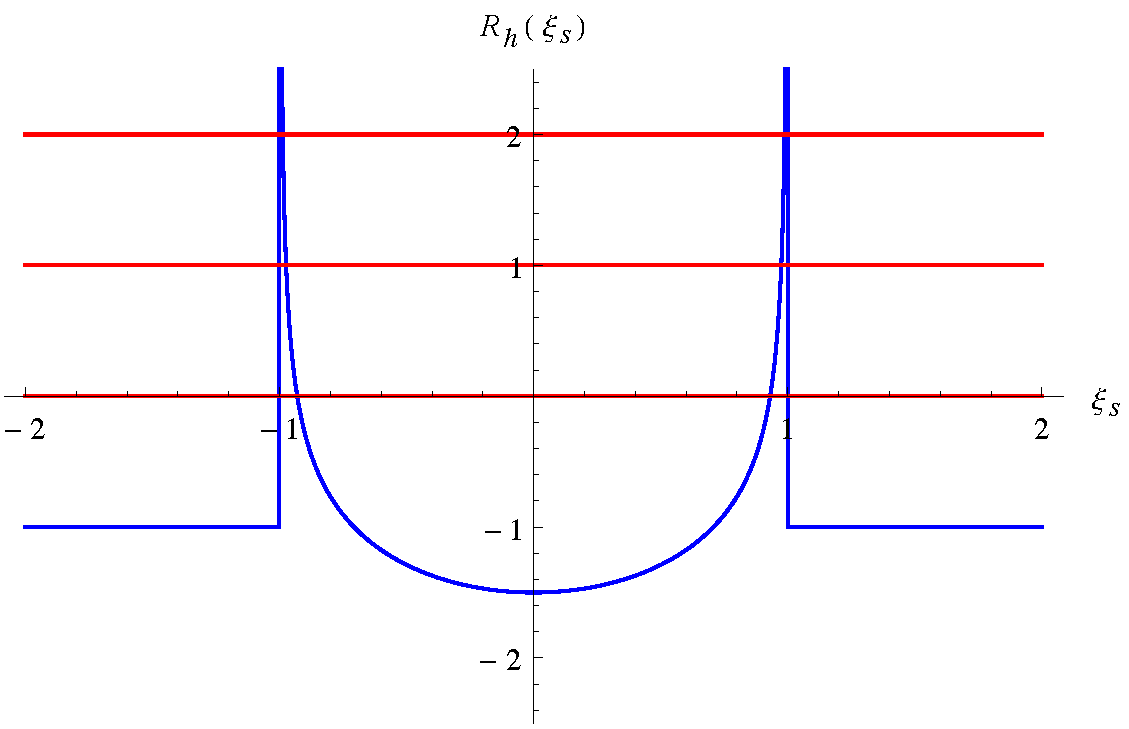
\includegraphics[scale=0.6]{Plots/ReRh.pdf}
\caption[Real part of the Regge trajectory function for the massless symmetric tensor exchange model]{Real part of $R_{h}(\xi_{s})$. The red lines correspond to $R_{h} = 0, 1, 2$. We have used $m_{a} m_{b} \alpha_{2} = 0.5$.}
\label{ReRhFig}
\end{figure}

\begin{figure}
\centering
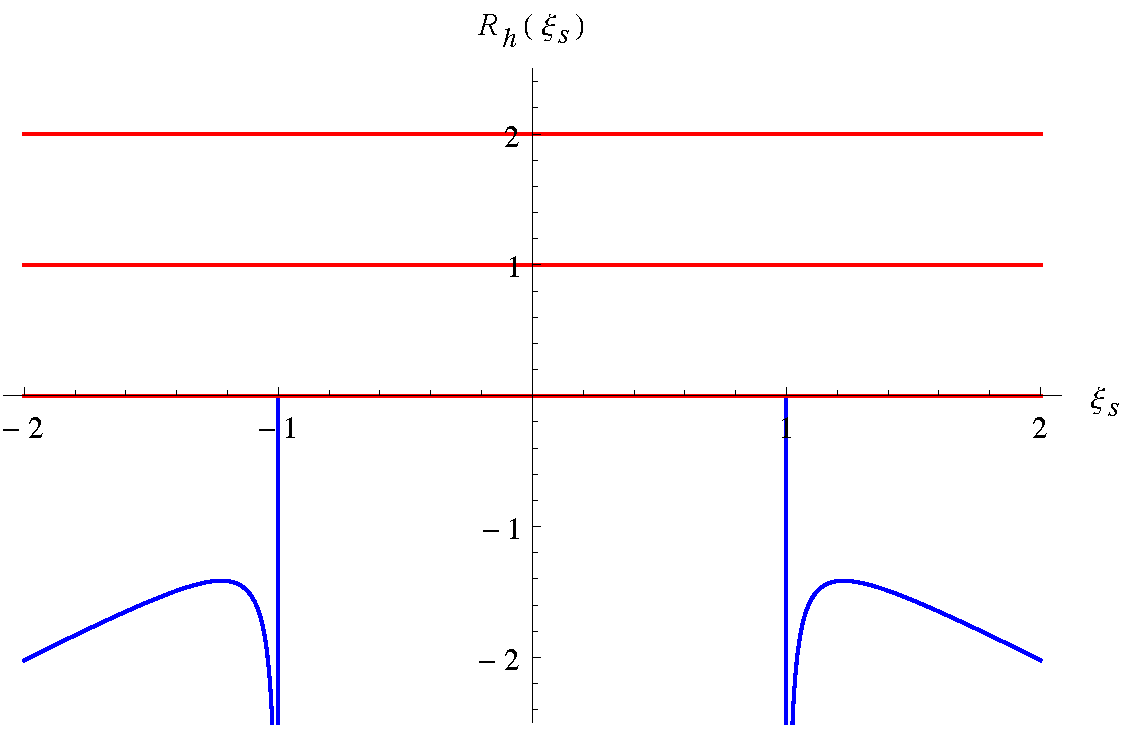
\includegraphics[scale=0.6]{Plots/ImRh.pdf}
\caption[Imaginary part of the Regge trajectory function for the massless symmetric tensor exchange model]{Imaginary part of $R_{h}(\xi_{s})$. The red lines correspond to $R_{h} = 0, 1, 2$. We have used $m_{a} m_{b} \alpha_{2} = 0.5$.}
\label{ImRhFig}
\end{figure}

Solving the singularity condition $J = R_{h}(s_{J}, u_{J})$ leads to
\begin{equation}
\begin{split}
	s_{J} = &{} m_{a}^{2} + m_{b}^{2} - \frac{t}{2} \\
	&+ 2 m_{a} m_{b} \sqrt{\left(1 - \frac{t}{4m_{a}^{2}} \right)\left(1 - \frac{t}{4m_{b}^{2}} \right)\left[ \frac{1}{2} + \left(1 + \sqrt{1 + \kappa} \right)^{-1} \right]}
\end{split}
\end{equation}
where
\begin{equation}
	\kappa = \frac{8 m_{a}^{2} m_{b}^{2} \alpha_{2}^{2}}{(J+1)^{2}} \left(1 - \frac{t}{4m_{a}^{2}} \right)\left(1 - \frac{t}{4m_{b}^{2}} \right)
\end{equation}
Using
\begin{equation}
	s_{J} + t + u_{J} = 2m_{a}^{2} + 2m_{b}^{2}
\end{equation}
we find
\begin{equation}
\begin{split}
	u_{J} = &{} m_{a}^{2} + m_{b}^{2} - \frac{t}{2} \\
	&- 2 m_{a} m_{b} \sqrt{\left(1 - \frac{t}{4m_{a}^{2}} \right)\left(1 - \frac{t}{4m_{b}^{2}} \right)\left[ \frac{1}{2} + \left(1 + \sqrt{1 + \kappa} \right)^{-1} \right]}
\end{split}
\end{equation}
In the two-body semiclassical eikonal approximation (\ref{2BodyEikonalJWKB}), we have
\begin{equation}
	\frac{s_{J}}{m_{a} m_{b}} \approx \frac{m_{a}^{2} + m_{b}^{2}}{m_{a} m_{b}} + 2 \left[ \frac{1}{2} + \left(1 + \sqrt{1 + \frac{8 m_{a}^{2} m_{b}^{2} \alpha_{2}^{2}}{(J + 1)^{2}}} \right)^{-1} \right]^{1/2} \label{sJTen4}
\end{equation}
Just like for the exchange of the massless vector, the expression for $s_{J}$ in (\ref{sJTen4}) is valid for any value of $\alpha_{2}$. Near $\alpha_{2} = 0$ we find
\begin{equation}
	s_{J} \approx m_{a}^{2} + m_{b}^{2} + 2 m_{a} m_{b} \left[1 - \frac{m_{a}^{2} m_{b}^{2} \alpha_{2}^{2}}{2(J + 1)^{2}} + \ldots \right]
\end{equation}
On the other hand, near $\alpha_{2} \rightarrow \infty$ we find
\begin{equation}
	s_{J} \approx m_{a}^{2} + m_{b}^{2} + 2 m_{a} m_{b} \left[ 1 - \frac{\sqrt{2} - 1}{\sqrt{2}} + \frac{(J + 1)}{4 m_{a} m_{b} \alpha_{2}} + \ldots \right]
\end{equation}
which is analogous to (\ref{StringSpec}).